%%%%%%%%%%%%%%%%%%%%%%%%%%%%%%%%%%%%%%%%%%%%%%%%%%%%%%%%%%%%%%%%%%%%%%
% LaTeX Example: Project Report
%
% Source: http://www.howtotex.com
%
% Feel free to distribute this example, but please keep the referral
% to howtotex.com
% Date: March 2011 
% 
%%%%%%%%%%%%%%%%%%%%%%%%%%%%%%%%%%%%%%%%%%%%%%%%%%%%%%%%%%%%%%%%%%%%%%
% How to use writeLaTeX: 
%
% You edit the source code here on the left, and the preview on the
% right shows you the result within a few seconds.
%
% Bookmark this page and share the URL with your co-authors. They can
% edit at the same time!
%
% You can upload figures, bibliographies, custom classes and
% styles using the files menu.
%
% If you're new to LaTeX, the wikibook is a great place to start:
% http://en.wikibooks.org/wiki/LaTeX
%
%%%%%%%%%%%%%%%%%%%%%%%%%%%%%%%%%%%%%%%%%%%%%%%%%%%%%%%%%%%%%%%%%%%%%%
% Edit the title below to update the display in My Documents
%\title{Project Report}
%
%%% Preamble
\documentclass[paper=a4, fontsize=11pt]{scrartcl}
\usepackage[T1]{fontenc}
\usepackage{fourier}
\usepackage[utf8]{inputenc}
\usepackage[spanish]{babel}															% English language/hyphenation
\usepackage[protrusion=true,expansion=true]{microtype}	
\usepackage{amsmath,amsfonts,amsthm} % Math packages
\usepackage[pdftex]{graphicx}	
\usepackage{url}
\usepackage{hyperref}

%%% Custom sectioning
\usepackage{sectsty}
\allsectionsfont{\normalfont\scshape}


%%% Custom headers/footers (fancyhdr package)
\usepackage{fancyhdr}
\pagestyle{fancyplain}
\fancyhead{}											% No page header
\fancyfoot[L]{}											% Empty 
\fancyfoot[C]{}											% Empty
\fancyfoot[R]{\thepage}									% Pagenumbering
\renewcommand{\headrulewidth}{0pt}			% Remove header underlines
\renewcommand{\footrulewidth}{0pt}				% Remove footer underlines
\setlength{\headheight}{13.6pt}


%%% Equation and float numbering
\numberwithin{equation}{section}		% Equationnumbering: section.eq#
\numberwithin{figure}{section}			% Figurenumbering: section.fig#
\numberwithin{table}{section}				% Tablenumbering: section.tab#


% Custom colors
\usepackage{color}
\definecolor{deepblue}{rgb}{0,0,0.5}
\definecolor{deepred}{rgb}{0.6,0,0}
\definecolor{deepgreen}{rgb}{0,0.5,0}

\usepackage{listings}

% Python style for highlighting
\newcommand\pythonstyle{\lstset{
language=Python,
basicstyle=\ttm,
otherkeywords={self},             % Add keywords here
keywordstyle=\ttb\color{deepblue},
emph={MyClass,__init__},          % Custom highlighting
emphstyle=\ttb\color{deepred},    % Custom highlighting style
stringstyle=\color{deepgreen},
% frame=tb,                         % Any extra options here
showstringspaces=false            % 
}}


% Python environment
\lstnewenvironment{python}[1][]
{
\pythonstyle
\lstset{#1}
}
{}

% Python for external files
\newcommand\pythonexternal[2][]{{
\pythonstyle
\lstinputlisting[#1]{#2}}}

% Python for inline
\newcommand\pythoninline[1]{{\pythonstyle\lstinline!#1!}}

%%% Maketitle metadata
\newcommand{\horrule}[1]{\rule{\linewidth}{#1}} 	% Horizontal rule

\title{
		%\vspace{-1in} 	
		\usefont{OT1}{bch}{b}{n}
		\normalfont \normalsize \textsc{Universidad Católica de San Pablo \\
		Maestría en Ciencia de la Computación \\
        Sistemas Inteligentes} \\ [25pt]
		\horrule{0.5pt} \\[0.4cm]
		\huge Máquina de Vectores de Soporte (SVM) \\
        Prof. Graciela Meza Lovón \\
		\horrule{2pt} \\[0.5cm]
}
\author{
		\normalfont 								\normalsize
        Palomino Paucar, Daniel Alfredo\\[-3pt]		\normalsize
        Noviembre 26, 2018 \\
        \url{https://bit.ly/2r7y556}
}
\date{}

%%% Begin document
\begin{document}
\maketitle

\newpage
\section{Preguntas de Teoría}

\textbf{Sea el conjunto $S={((1,6),-1), ((4,9),-1), ((4,6),-1), ((5,1),1), ((9,5),1), ((9,1),1)}$ y un conjunto de cuatro hiperplanos $H = {H_1, H_2, H_3, H_4}$ definidos como: $H_1: x_1 - x_2 -1 = 0$, $H_2: 2x_1 - 7x_2 +32 =0$, $H_3: \sqrt{\frac{1}{2}}x_1 - \sqrt{\frac{1}{2}}x_2 - \sqrt{\frac{1}{2}} = 0$, $H_4: 2x_1 - 7x_2 -32 = 0$}

\begin{enumerate}
    \item Usando cualquier lenguaje de programación grafique $S,\ H_1,\ H_2,\ H_3\ y\ H_4$.
    
    \textbf{Respuesta:}
    
    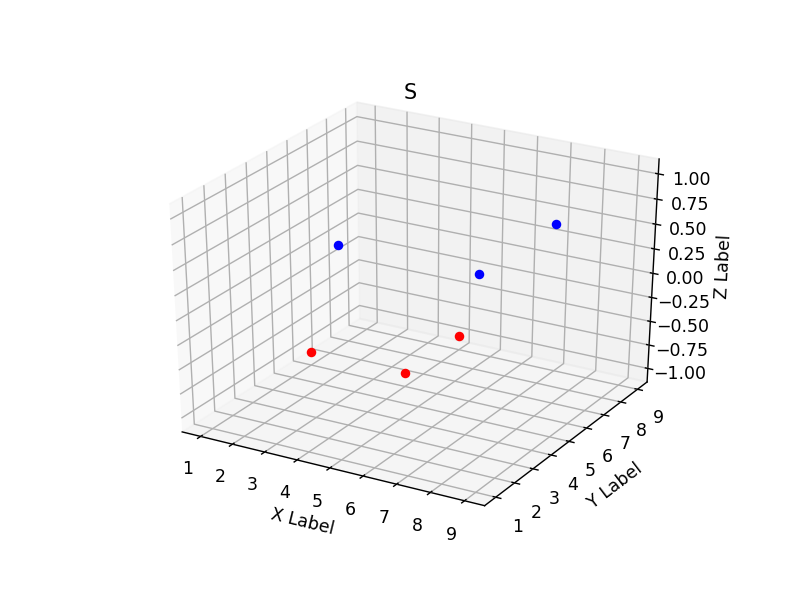
\includegraphics[scale=0.4]{S}
    
    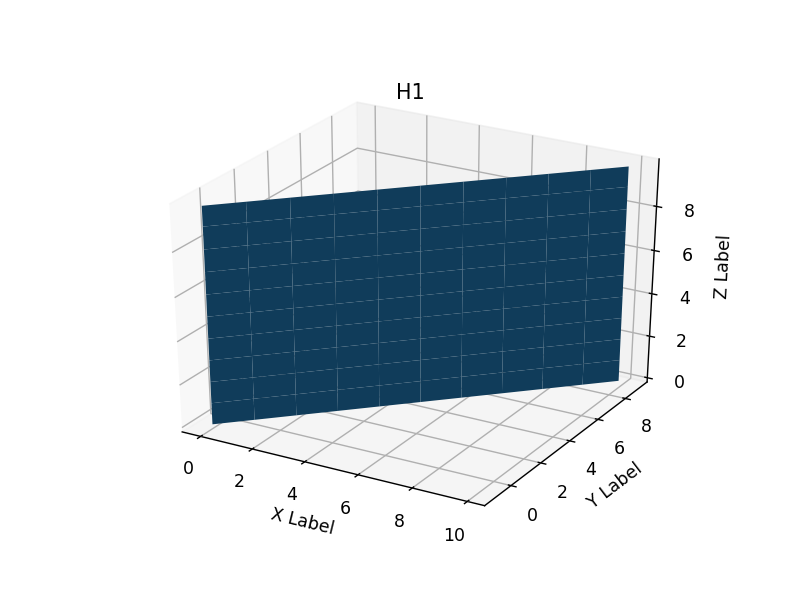
\includegraphics[scale=0.4]{H1}
    
    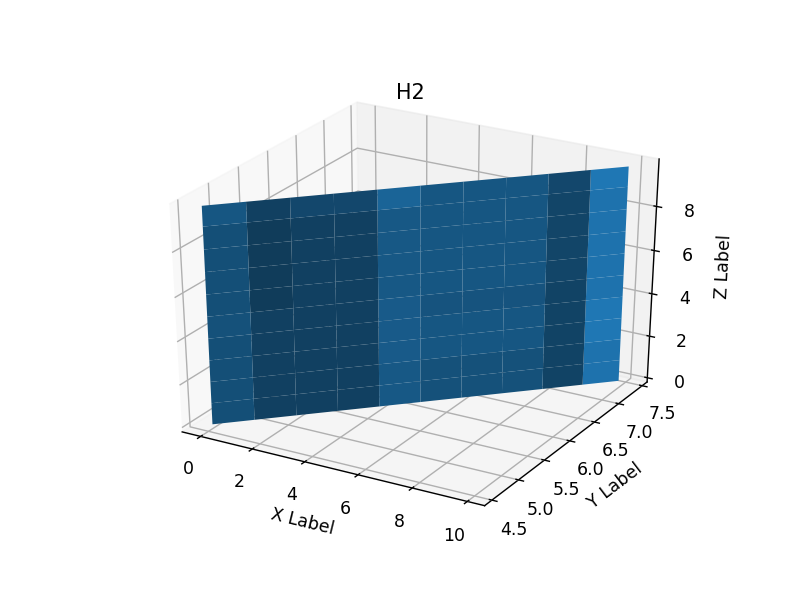
\includegraphics[scale=0.4]{H2}
    
    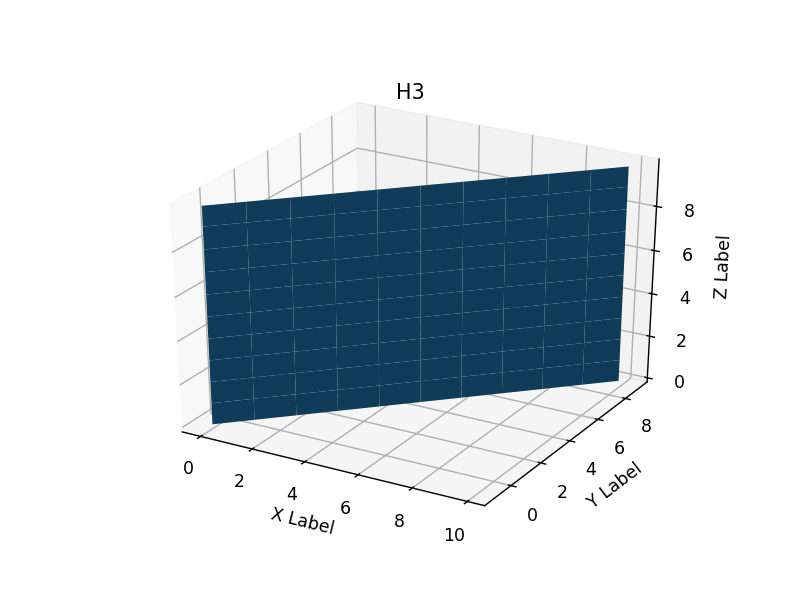
\includegraphics[scale=0.4]{H3}
    
    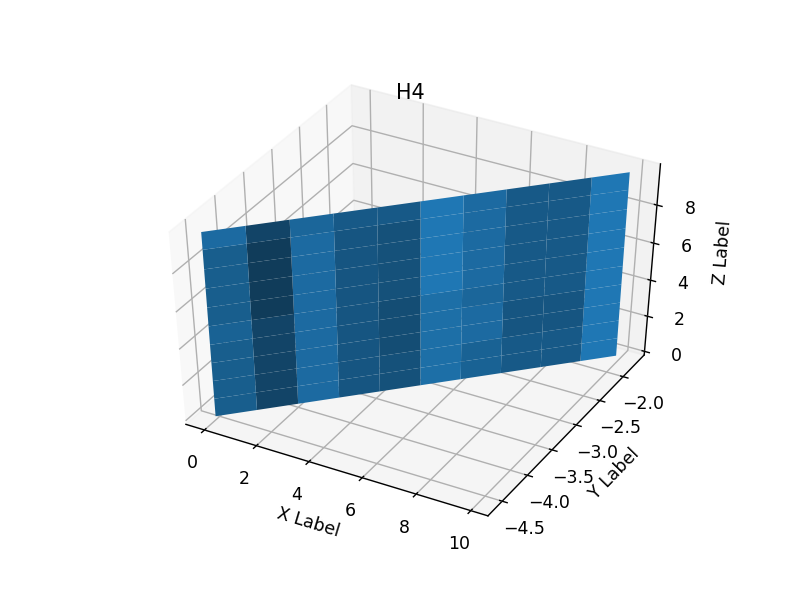
\includegraphics[scale=0.4]{H4}
    
    \item Encuentre  los parámetros $w$ y $b$ que definen los hiperplanos $H_1,\  H_2,\ H_3\ y\ H_4$, y luego determine para $H_1,\  H_2,\ H_3\ y\ H_4$ si son hiperplanos de separación. Fundamente.
    
    \textbf{Respuesta:}
    
    Dadas la ecuación vectorial de un hiperplano: $W.X + b = 0$, se tiene al extender la ecuación: $w_1.x_1 + w_2.x_2 + w_3.w_3 +b = 0$.
    
    Dando la forma a la ecuaciones dadas:
    
    \begin{enumerate}
        \item $H_1:$
                $$ x_1 - x_2 -1 = 0 $$
                $$ (1,-1,0).X - 1 =0 $$
                Entonces: $$W = (1,-1,0) \wedge b=-1$$
                
                Graficando:
                
                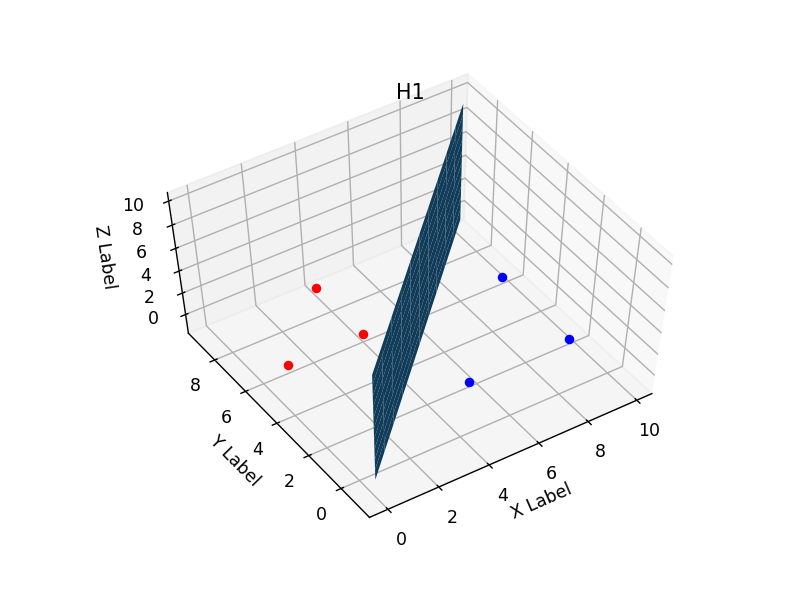
\includegraphics[scale=0.4]{S_H1}
                
                Por lo tanto $H_1$: Sí es un hiperplano de separación.
                
        \item $H_2:$
                $$ 2x_1 - 7x_2 +32 =0 $$
                $$ (2,-7,0).X +32 =0 $$
                Entonces: $$W=(2,-7,0) \wedge b=32$$
                
                Graficando:
                
                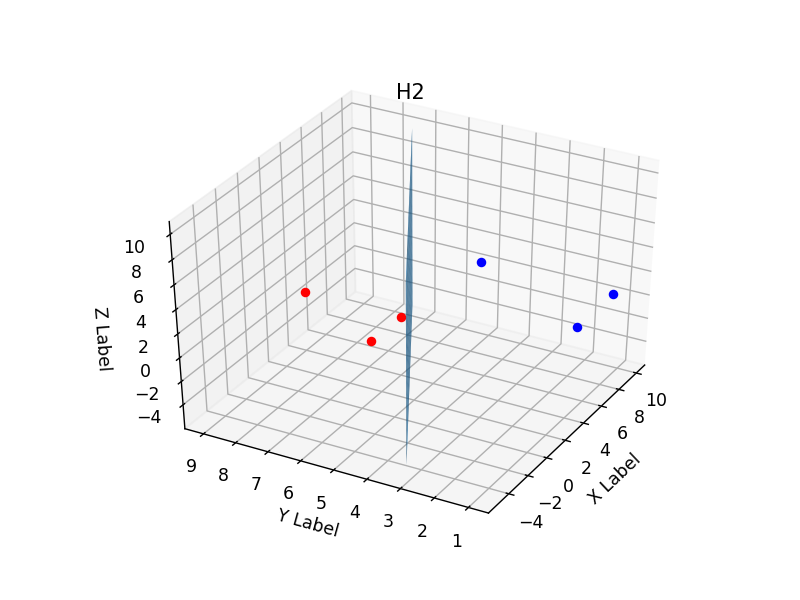
\includegraphics[scale=0.4]{S_H2}
                
                Por lo tanto $H_2$: Sí es un hiperplano de separación.
                
        \item $H_3:$
                $$ \sqrt{\frac{1}{2}}x_1 - \sqrt{\frac{1}{2}}x_2 - \sqrt{\frac{1}{2}} = 0 $$
                $$ (1,-1,0).X -1 =0 $$
                Entonces: $$W = (\sqrt{\frac{1}{2}},-\sqrt{\frac{1}{2}},0) \wedge b=-\sqrt{\frac{1}{2}}$$
                
                Graficando:
                
                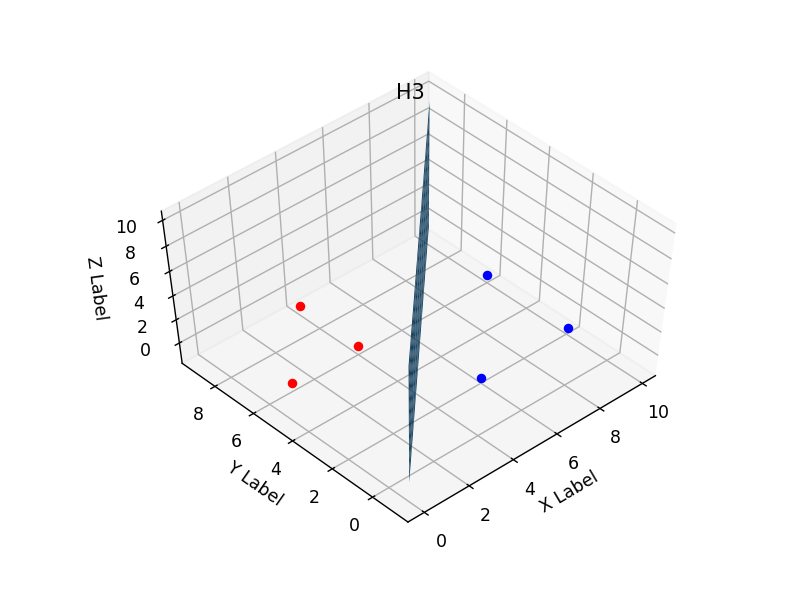
\includegraphics[scale=0.4]{S_H3}
                
                Por lo tanto $H_3$: Sí es un hiperplano de separación.
                
        \item $H_4:$
                $$ 2x_1 - 7x_2 -32 = 0 $$
                $$ (2,-7,0).X - 32=0 $$
                Entonces: $$W=(2,-7,0) \wedge b=-32$$
                
                Graficando:
                
                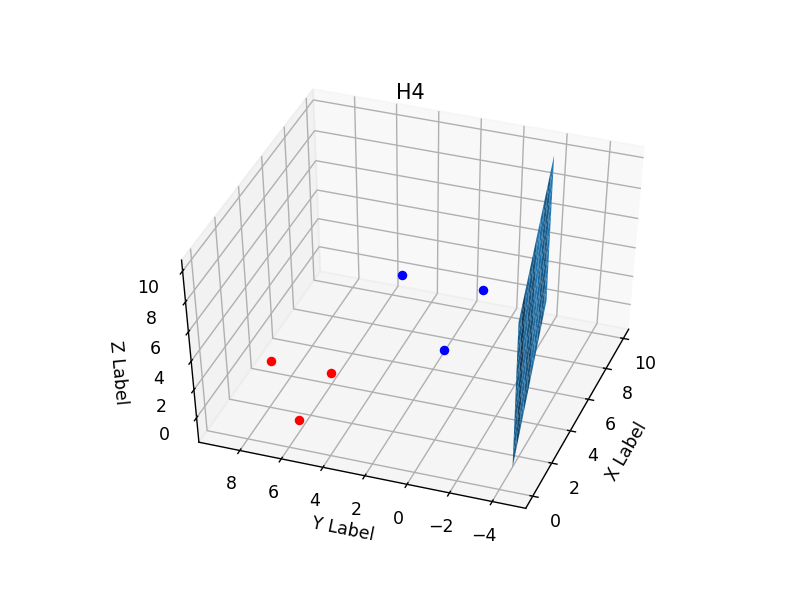
\includegraphics[scale=0.4]{S_H4}
                
                Por lo tanto $H_4$: No es un hiperplano de separación.\\
                
    \end{enumerate}
    
    
    \item En el conjunto $H$, ¿cuántos hiperplanos iguales existen?. En el caso de que existan ¿cuáles son éstos? Fundamente.\\
    
    \textbf{Respuesta:}
    
    Existen 2 hiperplanos iguales $H_1\ y\ H_3$, dado que si a la ecuación de $H_3$ la dividimos entre $\sqrt{\frac{1}{2}}$ tendríamos la misma ecuación que $H_1$.\\
    
    
    \item Calcule el margen $\tau$ para cada hiperplano de separación. Luego, suponga que el conjunto $H$ contiene al hiperplano óptimo  $H^*$, ¿cuál sería $H^*$? Fundamente.\\
    
    \textbf{Respuesta:}
    
    \begin{enumerate}
        \item $H_1$:
                $$\tau_1 = 2.1213$$
                
        \item $H_2$:
                $$\tau_2 = 0.2742$$
                
        \item $H_3$:
                $$\tau_3 = 2.1213$$
    \end{enumerate}
    
    De acuerdo a los datos calculados, si el hiperplano $H^*$ existiera en el conjunto $H$, este sería $H_1$ o $H_3$ (pues representan el mismo plano), dado que poseen el $\tau$ con mayor valor.
    
    \item ¿Cuáles son los vectores de soporte del hiperplano $H^*$ escogido en la pregunta anterior?. Fundamente. (No necesita encontrar los valores $\alpha$)\\
    
    \textbf{Respuesta:}
    
    Los vectores de soporte del hiperplano óptimo elegido ($H_1$ o $H_3$)serían:
    
    $$(4,6,-1),\ (5,1,1),\ (9,5,1)$$
    
    pues se encuentran en el margen óptimo, teniendo cada vector el $\tau$ mínimo de $2.1313$.\\
    
    \item Demuestre la primera condición KKT, i.e. (Ec. 7 de las diapositivas) $\frac{\partial L}{\partial w}(w^*, b^*, \alpha) = w^* - \sum_{i=1}^{m}\alpha_iy(i)x^{i}$\\
    
    \textbf{Respuesta:}
    
    Sea: $$L = \frac{1}{2}W.W^T - \sum_{i=1}^{m}\alpha_i[y^{(i)}(W^{T}X^{(i)} + b) - 1]$$
    
    Expandiendo los términos:
    
    $$L = \frac{1}{2}W.W^T - \sum_{i=1}^{m}\alpha_i[y^{(i)}W^{T}X^{(i)}] - \sum_{i=1}^{m}\alpha_i[y^{(i)}b] + \sum_{i=1}^{m}\alpha_i$$
    
    Para encontrar los $W*, b^*, \alpha^*$ óptimo, necesitamos derivar respecto de los parámetros, lo cual se describe en la ecuación 1:
    
    $$\frac{\partial L(W^*, b^*, \alpha^* )}{\partial w_i}=0, i=1,...,n$$
    
    Entonces, derivando $L$ respecto de $w_i$ tenemos:
    
    $$\frac{\partial L(W^*, b^*, \alpha^* )}{\partial w_i}=\frac{\partial (\frac{1}{2}W.W^T - \sum_{i=1}^{m}\alpha_i[y^{(i)}W^{T}X^{(i)}] - \sum_{i=1}^{m}\alpha_i[y^{(i)}b] + \sum_{i=1}^{m}\alpha_i)}{\partial w_i}$$
    
    Separando los términos de la derecha:
    
    $$\frac{\partial L(W^*, b^*, \alpha^* )}{\partial w_i}=\frac{\partial (\frac{1}{2}W.W^T)}{\partial w_i} - \frac{\partial (\sum_{i=1}^{m}\alpha_i[y^{(i)}W^{T}X^{(i)}])}{\partial w_i} - \frac{\partial (\sum_{i=1}^{m}\alpha_i[y^{(i)}b])}{\partial w_i}+ \frac{\partial (\sum_{i=1}^{m}\alpha_i)}{\partial w_i}$$
    
    El tercer y cuarto término de la derecha no depende de $w_i$, por lo tanto al derevirase desapareceran:
    
    $$\frac{\partial L(W^*, b^*, \alpha^* )}{\partial w_i}=\frac{\partial (\frac{1}{2}W.W^T)}{\partial w_i} - \frac{\partial (\sum_{i=1}^{m}\alpha_i[y^{(i)}W^{T}X^{(i)}])}{\partial w_i}$$
    
    Finalmente calculando la derivada parcial:
    
    $$\frac{\partial L}{\partial w}(w^*, b^*, \alpha) = w^* - \sum_{i=1}^{m}\alpha_iy(i)x^{i}=0$$
    
    Quedando demostrado la ecuación 7 de las diapositivas.\\
    

\textbf{Sea el conjunto $N = {((1,6),-1), ((4,9),-1), ((4,6),-1), ((5,1),1), ((9,1),1), ((0,3),1), ((2,2),-1), ((3,1),-1)}$ y el hiperplano $H_1$ definido anteriormente.}\\

    \item Usando cualquier lenguaje de programación grafique $N$ y $H_5$.
    
    \textbf{Respuesta:}
    
    Graficando:
        
    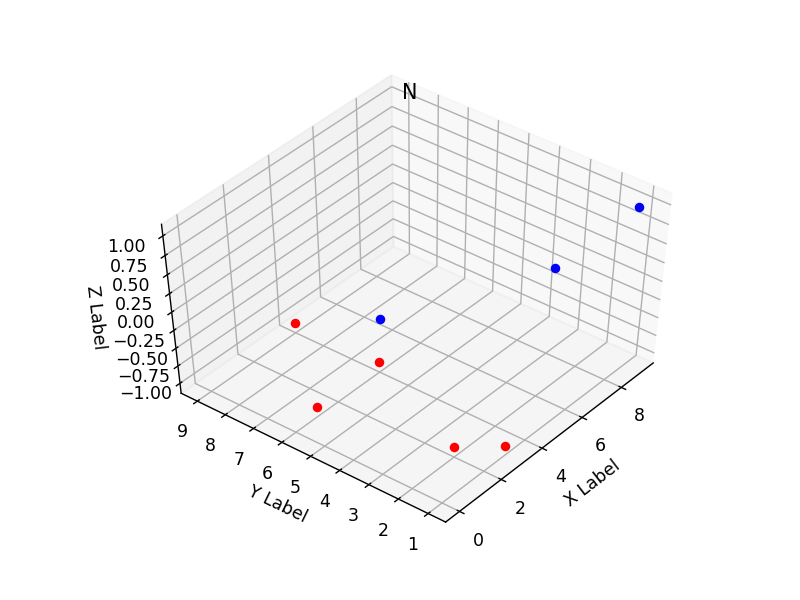
\includegraphics[scale=0.4]{N}
    
    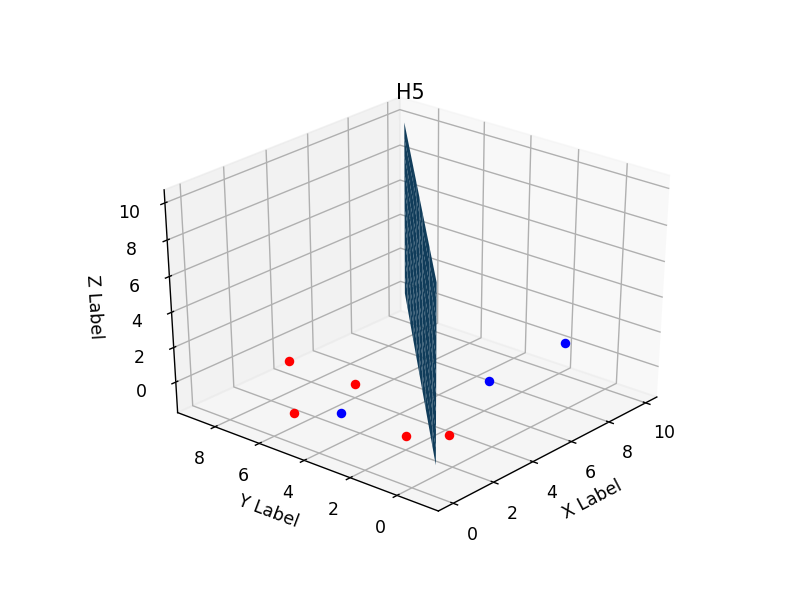
\includegraphics[scale=0.4]{N_H5}
    
    \item Identifique los ejemplos que son separables y los que no lo son. Luego, determine los ejemplos que son clasificados correctamente y los que no.
    
    \textbf{Respuesta:}
    
    Para que un vector sea separable debe cumplir:
    
    $$y_i(W^TX)\geq 1$$
    
    Por lo tanto haciendo los cálculos para los ejemplos del espacion $N$ y el hiperplano $H_5$:
    
    \begin{enumerate}
        \item $((1,6),-1)$: 5
        \item $((4,9),-1)$: 5
        \item $((4,6),-1)$: 2
        \item $((5,1),1)$: 4
        \item $((9,1),1)$: 8
        \item $((0,3),1)$: -3
        \item $((2,2),-1)$: 0
        \item $((3,1),-1)$: -2
    \end{enumerate}
    
    \newpage
    
    Por lo tanto: 
    Los ejemplos separables son:\\
    ${((1,6),-1), ((4,9),-1), ((4,6),-1), ((5,1),1), ((9,1),1)}$
    
    y los no separables son:\\
    ${((0,3),1), ((2,2),-1), ((3,1),-1)}$
    
    Así mismo, los ejemplos clasificados correctamente son:\\
    ${((1,6),-1), ((4,9),-1), ((4,6),-1), ((5,1),1), ((9,1),1)}, ((2,2),-1)$
    
    y los no clasficados correctamente son:\\
    ${((0,3),1), ((3,1),-1)}$\\
    
    \item Calcule la holgura de los ejemplos no separables.
    
    \textbf{Respuesta:}
    
    Dado que:
    
    $$y_i(W^TX)\geq 1 - \epsilon_i$$
    
    Se tendrá para los ejemplos no separables ${((0,3),1), ((2,2),-1), ((3,1),-1)}$:
    
    \begin{enumerate}
        \item $((0,3),\ 1)$: $\epsilon_i = 4$
        \item $((2,2),-1)$: $\epsilon_i = 1$
        \item $((3,1),-1)$: $\epsilon_i = 3$
    \end{enumerate}

\end{enumerate}
\newpage
\section{Preguntas de Investigación}

\begin{enumerate}
    \item Explique el significados de la constante $C$ en el término $C\sum_{i=1}\epsilon_i$ que se agrega a la función objetivo en el caso de ejemplos casi linealmente separables. Luego, explique la influencia de $C$ en la capacidad de generalización de una SVM.
    
    \textbf{Respuesta:}
    
    El parámetro $C$ está asociado al mejoramiento de la generalización del sistema evitando el overfitting, es análogo al parámetro de regularización usando en redes neuronales.
    
    El parámetro $C$ le dice al sistema SVM que tanto quiere que se evite el error de clasficación (misclassifying) por cada ejemplo de entrenamiento. 
    
    Para valores grandes de $C$, la optimización elegirá un hiperplano de margen angosto si es que ese hiperplano realiza un mejor trabajo en clasificar correctamente todos los ejemplos de entrenamiento.
    
    Por el contrario, un valor muye pequeño de $C$ causará que sistema busque un hiperplano de margen amplio, incluso si ese hiperplano clasifica incorrectamente más puntos.
    
    \item Describa el significado del parámetro $\gamma$ en el kernel gaussiano. Luego, explique la influencia de $\gamma$ en la capacidad de generalización de una SVM.
    
    \textbf{Respuesta:}
    
    El parámetro $\gamma$ es el parámetro libre de la función base del radio gausiano.
    
    Un valor pequeño de $\gamma$ significa una función gaussiana con una varianza grande, así que la influencia de $x_j$ es más grande hacia $x_i$. Es decir, si $x_j$ es un vector de soporte, un valor pequeño de $\gamma$ implica que la clase de este vector de soporte tendrá influencia en decidir la clase del vector $x_i$ incluso si la distancia entre ellos es grande.
    
    Por el contrario, si $\gamma$ tiene un valor muy grande entonces la varianza será pequeña, lo que implica que el vector de soporte no tendrá una influencia importante sobre vectores más alejados.
    
\end{enumerate}

\newpage
\section{Implementación}

\begin{enumerate}
    \item Usando Scikit-learn de Python, implemente (comente su código) una svm que clasifique el conjunto de datos (por definir).
    
    \textbf{Implementación:}
    
    Como no se ha incluído el dataset, he propuesto trabajar el presente ejercicio con el siguiente dataset (Iris Flower):\\
    \url{https://archive.ics.uci.edu/ml/machine-learning-databases/iris/iris.data}\\
    
    \textbf{Lectura de Dataset}
    
    \begin{python}
    import numpy as np  
    import matplotlib.pyplot as plt  
    import pandas as pd
    
    url = "https://archive.ics.uci.edu/ml/machine-learning-databases"
          "/iris/iris.data"
    # Asignar columnas al Dataset para su posterior lectura
    colnames = ['sepal-length', 'sepal-width', 
                'petal-length', 'petal-width', 'Class']
    # Lectura del Dataset usando pandas
    irisdata = pd.read_csv(url, names=colnames)
    \end{python}
    
    \textbf{Exploración de Datos}
    
    \begin{python}
    # Dimensiones del Dataset
    irisdata.shape
    # Descripción del Dataset
    irisdata.head()
    \end{python}
    
    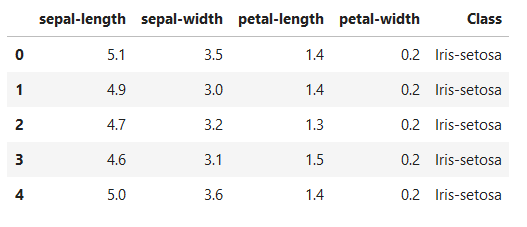
\includegraphics[scale=0.8]{df1_head}
    \newpage
    \textbf{Preprocesamiento}
    
    \begin{python}
    # Separación de las columnas del dataset para crear los valores de entrada
    # y el valor de salida
    X = irisdata.drop('Class', axis=1)  
    y = irisdata['Class'] 
    # Separación del dataset en valores de entranemiento y testeo
    from sklearn.model_selection import train_test_split  
    X_train, X_test, y_train, y_test = train_test_split(X, y, test_size = 0.20)
    \end{python}
    
    \textbf{Entrenamiento}
    
    \begin{python}
    from sklearn.svm import SVC
    # Elección del Kernel: linear
    svclassifier = SVC(kernel='linear')
    # Ejecución del entrenamiento
    svclassifier.fit(X_train, y_train)
    \end{python}
    
    \textbf{Predicción y Validación}
    
    \begin{python}
    # Predicción usando los valores de testeo
    y_pred = svclassifier.predict(X_test)
    from sklearn.metrics import classification_report, confusion_matrix
    # Creación de la matriz de confusión
    print(confusion_matrix(y_test,y_pred))
    # Creación de reporte de resultados
    print(classification_report(y_test,y_pred))
    \end{python}
    
    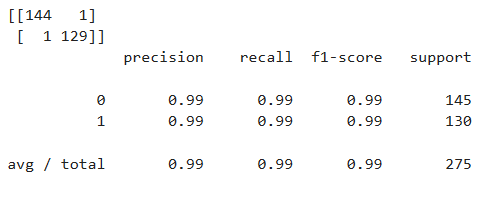
\includegraphics[scale=0.8]{df1_results}
    \newpage
    \item Experimente y muestre resultados usando diferentes valores para los parámetros de los kernels: lineal, polinomial, gaussiano, y el parámetro $C$. Los resultados deben ser mostrados en el documento pdf.
    
    \textbf{Implementación:}
    
    Como no se ha incluído el dataset, he propuesto trabajar el presente ejercicio con el siguiente dataset (Iris Flower): \url{https://archive.ics.uci.edu/ml/machine-learning-databases/iris/iris.data}\\
    
    \textbf{Lectura de Dataset}
    
    \begin{python}
    import numpy as np  
    import matplotlib.pyplot as plt  
    import pandas as pd
    
    url = "https://archive.ics.uci.edu/ml/machine-learning-databases"
          "/iris/iris.data"
    # Asignar columnas al Dataset para su posterior lectura
    colnames = ['sepal-length', 'sepal-width', 
                'petal-length', 'petal-width', 'Class']
    # Lectura del Dataset usando pandas
    irisdata = pd.read_csv(url, names=colnames)
    \end{python}
    
    \textbf{Exploración de Datos}
    
    \begin{python}
    # Descripción del Dataset
    bankdata.head()
    \end{python}
    
    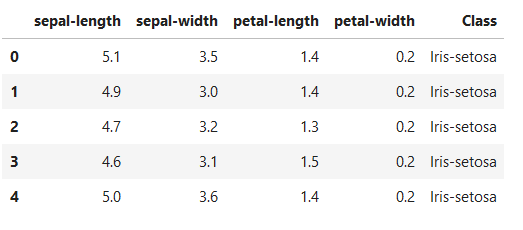
\includegraphics[scale=0.8]{df2_head}
    \newpage
    \textbf{Preprocesamiento}
    
    \begin{python}
    # Separación de las columnas del dataset para crear los valores de entrada
    # y el valor de salida
    X = irisdata.drop('Class', axis=1)  
    y = irisdata['Class'] 
    # Separación del dataset en valores de entranemiento y testeo
    from sklearn.model_selection import train_test_split  
    X_train, X_test, y_train, y_test = train_test_split(X, y, test_size = 0.20) 
    \end{python}
    
    \textbf{Lineal}
    
    \textbf{Entrenamiento}
    
    \begin{python}
    from sklearn.svm import SVC
    # Elección del Kernel: linear Y parámetro C=2.0
    svclassifier = SVC(kernel='linear', C=2.0)
    # Ejecución del entrenamiento
    svclassifier.fit(X_train, y_train)
    \end{python}
    
    \textbf{Predicción y Validación}
    
    \begin{python}
    # Predicción usando los valores de testeo
    y_pred = svclassifier.predict(X_test)
    from sklearn.metrics import classification_report, confusion_matrix
    # Creación de la matriz de confusión
    print(confusion_matrix(y_test,y_pred))
    # Creación de reporte de resultados
    print(classification_report(y_test,y_pred))
    \end{python}
    
    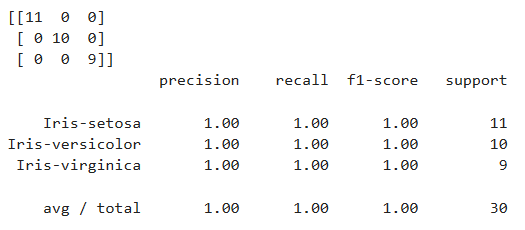
\includegraphics[scale=0.8]{df2_results_linear}
    \newpage
    \textbf{Polinomial}
    
    \textbf{Entrenamiento}
    
    \begin{python}
    from sklearn.svm import SVC
    # Elección del Kernel: poly Y parámetro C=0.5
    svclassifier = SVC(kernel='poly', degree=8, C=0.5)
    # Ejecución del entrenamiento
    svclassifier.fit(X_train, y_train)
    \end{python}
    
    \textbf{Predicción y Validación}
    
    \begin{python}
    # Predicción usando los valores de testeo
    y_pred = svclassifier.predict(X_test)
    from sklearn.metrics import classification_report, confusion_matrix
    # Creación de la matriz de confusión
    print(confusion_matrix(y_test,y_pred))
    # Creación de reporte de resultados
    print(classification_report(y_test,y_pred))
    \end{python}
    
    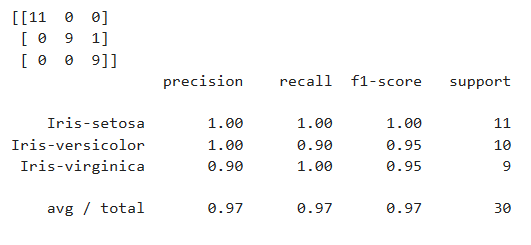
\includegraphics[scale=0.8]{df2_results_poly}
    
    \textbf{Gaussiano}
    
    \textbf{Entrenamiento}
    
    \begin{python}
    from sklearn.svm import SVC
    # Elección del Kernel: rbf
    svclassifier = SVC(kernel='rbf')
    # Ejecución del entrenamiento
    svclassifier.fit(X_train, y_train)
    \end{python}
    \newpage
    \textbf{Predicción y Validación}
    
    \begin{python}
    # Predicción usando los valores de testeo
    y_pred = svclassifier.predict(X_test)
    from sklearn.metrics import classification_report, confusion_matrix
    # Creación de la matriz de confusión
    print(confusion_matrix(y_test,y_pred))
    # Creación de reporte de resultados
    print(classification_report(y_test,y_pred))
    \end{python}
    
    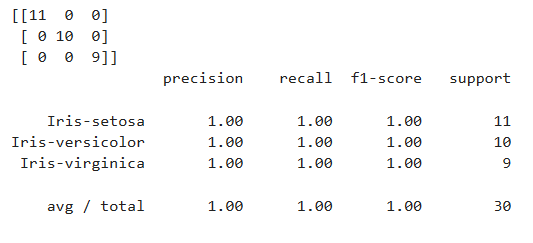
\includegraphics[scale=0.8]{df2_results_gaussian}
    
    \item Dentro de la sección de Implementación incluya una subsección donde indique las instrucciones para ejecutar el código.
    
    \textbf{Implementación:}
    
    La presente implementación ha sido realizada en python 3.6 usando anaconda y jupyter-lab como herramientas de virtualización y visualización.
    
    El notebook desarrollado que incluye todos los pasos descritos, así como los datasets, ha sido publicado en mi cunta de github:\\
    
    \url{https://github.com/dpalominop/SistemasInteligentes/blob/master/semana7/homework/svm.ipynb}
    
\end{enumerate}

%%% End document
\end{document}